  %%%%%%%%%%%%%%%%%%%%%%%%%%%%%%%%%%%%%%% -*- coding: utf-8; mode: latex -*- %%
  %
%%%%%                       CHAPTER
 %%%
  %

% $Id: 5100-omnis-voluptas.tex,v 1.1 2007/11/23 09:52:44 david Exp $
% $Log: 5100-omnis-voluptas.tex,v $
% Revision 1.1  2007/11/23 09:52:44  david
% *** empty log message ***
%
%

  %%%%%%%%%%%%%%%%%%%%%%%%%%%%%%%%%%%%%%%%%%%%%%%%%%%%%%%%%%%%%%%%%%%%%%%%%%%%%
  %
%%%%%                    HEAD MATTER
 %%%
  %

\chapter{Evaluation}
%\addcontentsline{lof}{chapter}{\thechapter\quad Nihil Molestiae}
%\addcontentsline{lot}{chapter}{\thechapter\quad Nihil Molestiae}
\label{ch:evaluation}

The solution \textit{Optimistic Concurrency Control with Snapshot Isolation on Semantic Related Group} (OCC) is built on top of the transactional framework~\cite{peiro2013maintaining} in the second version of Hop-HDFS (PCC). The goal of this chapter is to prove that our OCC model performs better than PCC. As a proof of concept, we implemented the OCC version for the operation \textit{mkdirs} and also give a detailed evaluation on it compared with the PCC version. For this purpose, we concern about the execution time (elapsed time) needed to finish all the concurrent tasks.

\section{Experimental Testbed}
\label{sec:testbed}

The MySQL Cluster consists of six data nodes connected by 1 Gigabit LAN. Each data node has an Intel Xeon X5660 CPU at 2.80GHz, and contributes 6 GB RAM (5 GB Data Memory + 1 GB Index Memory) separately. Therefore, the total available memory for the cluster is 36 GB. The number of data replicas is 2. The maximum concurrent transactions is 10000 for each data node, and the inactive timeout for each transaction is 5 seconds. 

\noindent To avoid any communication overhead caused by RPC connections and serialization, we run the NameNode and Clients on the same machine with Intel i7-4770T CPU at 2.50GHz and 16 GB RAM. This machine is connected with the MySQL Cluster data nodes by 100 Megabits LAN.

  %%%%%%%%%%%%%%%%%%%%%%%%%%%%%%%%%%%%%%%%%%%%%%%%%%%%%%%%%%%%%%%%%%%%%%%%%%%%%
  %
%%%%%                      SECOND SECTION
 %%%
  %

\section{Parent Directory Contention Assessment}
\label{sec:ww}

This experiment is the same as described in Section~\ref{sec:pdcassement}, but we expand it to include the results with OCC. See Figure~\ref{fig:hdfsPCCOCCparentDiragram} for the workload visual diagram. Here we have a full performance comparison here among HDFS, PCC and OCC.

\begin{figure}[ht]
	\centering
	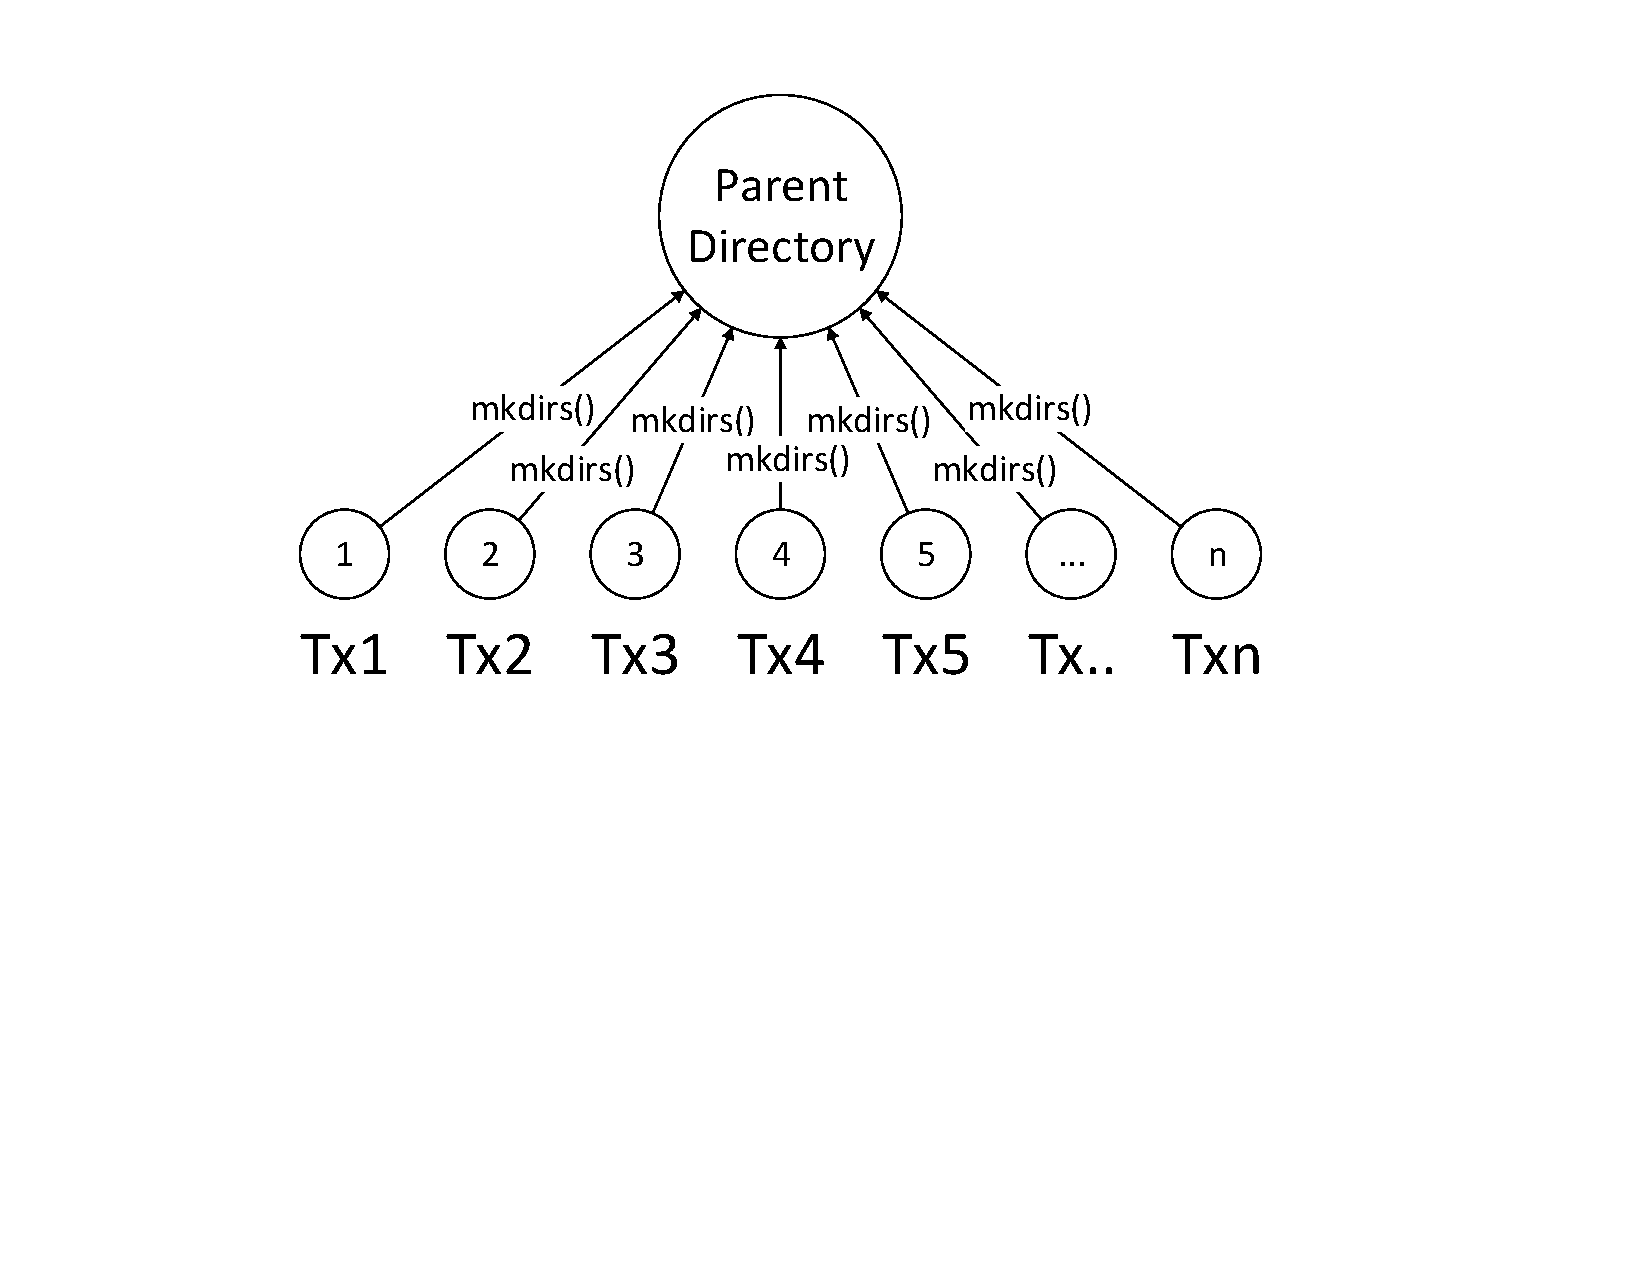
\includegraphics[scale=0.6]{figs/ww.pdf}
	\caption{Workload of Parent Directory Contention Assessment}
	\label{fig:hdfsPCCOCCparentDiragram}
\end{figure}

\noindent From Figure~\ref{fig:hdfsPCCOCCparent} and Table~\ref{table:hdfsPCCOCCparent}, we can see that OCC significantly outperforms PCC by almost 70 \% on this concurrent write-write parent directory contention workload. Under heavy workload, the execution time is just 1.3 times of HDFS. Remember that this is just a single NameNode performance test. We believe that OCC can greatly outperform HDFS in our multiple NameNodes architecture.

\begin{figure}[ht]
	\centering
	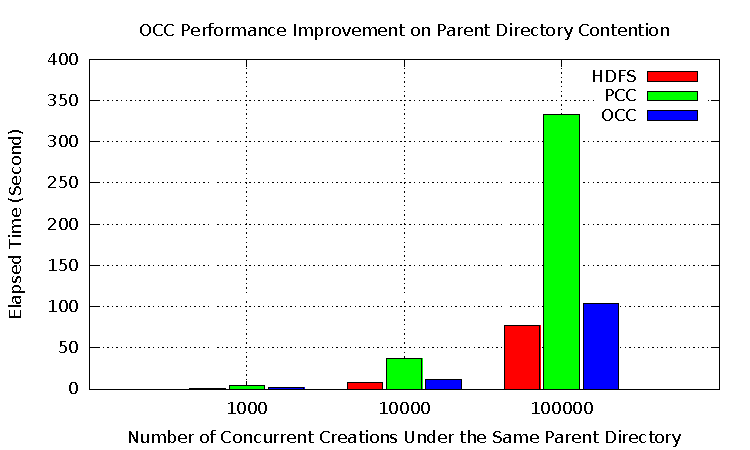
\includegraphics[width=\linewidth]{figs/hdfs_pcc_occ_parent.pdf}
	\caption{OCC Performance Improvement on Parent Directory Contention}
	\label{fig:hdfsPCCOCCparent}
\end{figure}

\begin{table}[ht]
	\centering
	\begin{tabular}{|c|c|c|c|}
		\hline
		\textbf{Num. of Concurrent Creation}                                                 & \textbf{1000}   & \textbf{10000}  & \textbf{100000} \\ \hline
		HDFS                                                                                 & 0.82s           & 7.83s           & 77.13s          \\ \hline
		PCC                                                                                  & 4.35s           & 36.74s          & 332.36s         \\ \hline
		OCC                                                                                  & 1.36s           & 12.01s          & 103.23s         \\ \hline
		PCC / HDFS                                                                           & 530.5\%         & 469.2\%         & 430.9\%         \\ \hline
		OCC / HDFS                                                                           & 165.9\%         & 153.4\%         & 133.8\%         \\ \hline
		\textbf{\begin{tabular}[c]{@{}c@{}}OCC Improvement: \\ (PCC-OCC) / PCC\end{tabular}} & \textbf{68.7\%} & \textbf{67.3\%} & \textbf{68.9\%} \\ \hline
	\end{tabular}
	\caption{OCC Performance Improvement on Parent Directory Contention}
	\label{table:hdfsPCCOCCparent}
\end{table}

\section{Read-Write Mixed Workload Assessment}

In this experiment, we did a test for a read-write mixed workload assessment while the parent directory is still the contention point for PCC. So we assume that OCC will still outperform PCC in this kind of workload. 

\noindent Similar to the experiment in Section~\ref{sec:ww}, we have 1000, 10000 and 100000 concurrent clients' operations running under the same parent directory. But in each task, half of them will do the metadata read operation \textit{getFileStatus()}, while the other half will do the write operation \textit{mkdirs()}. See Figure~\ref{fig:rwWorkload} for a visual reference.

\begin{figure}[ht]
	\centering
	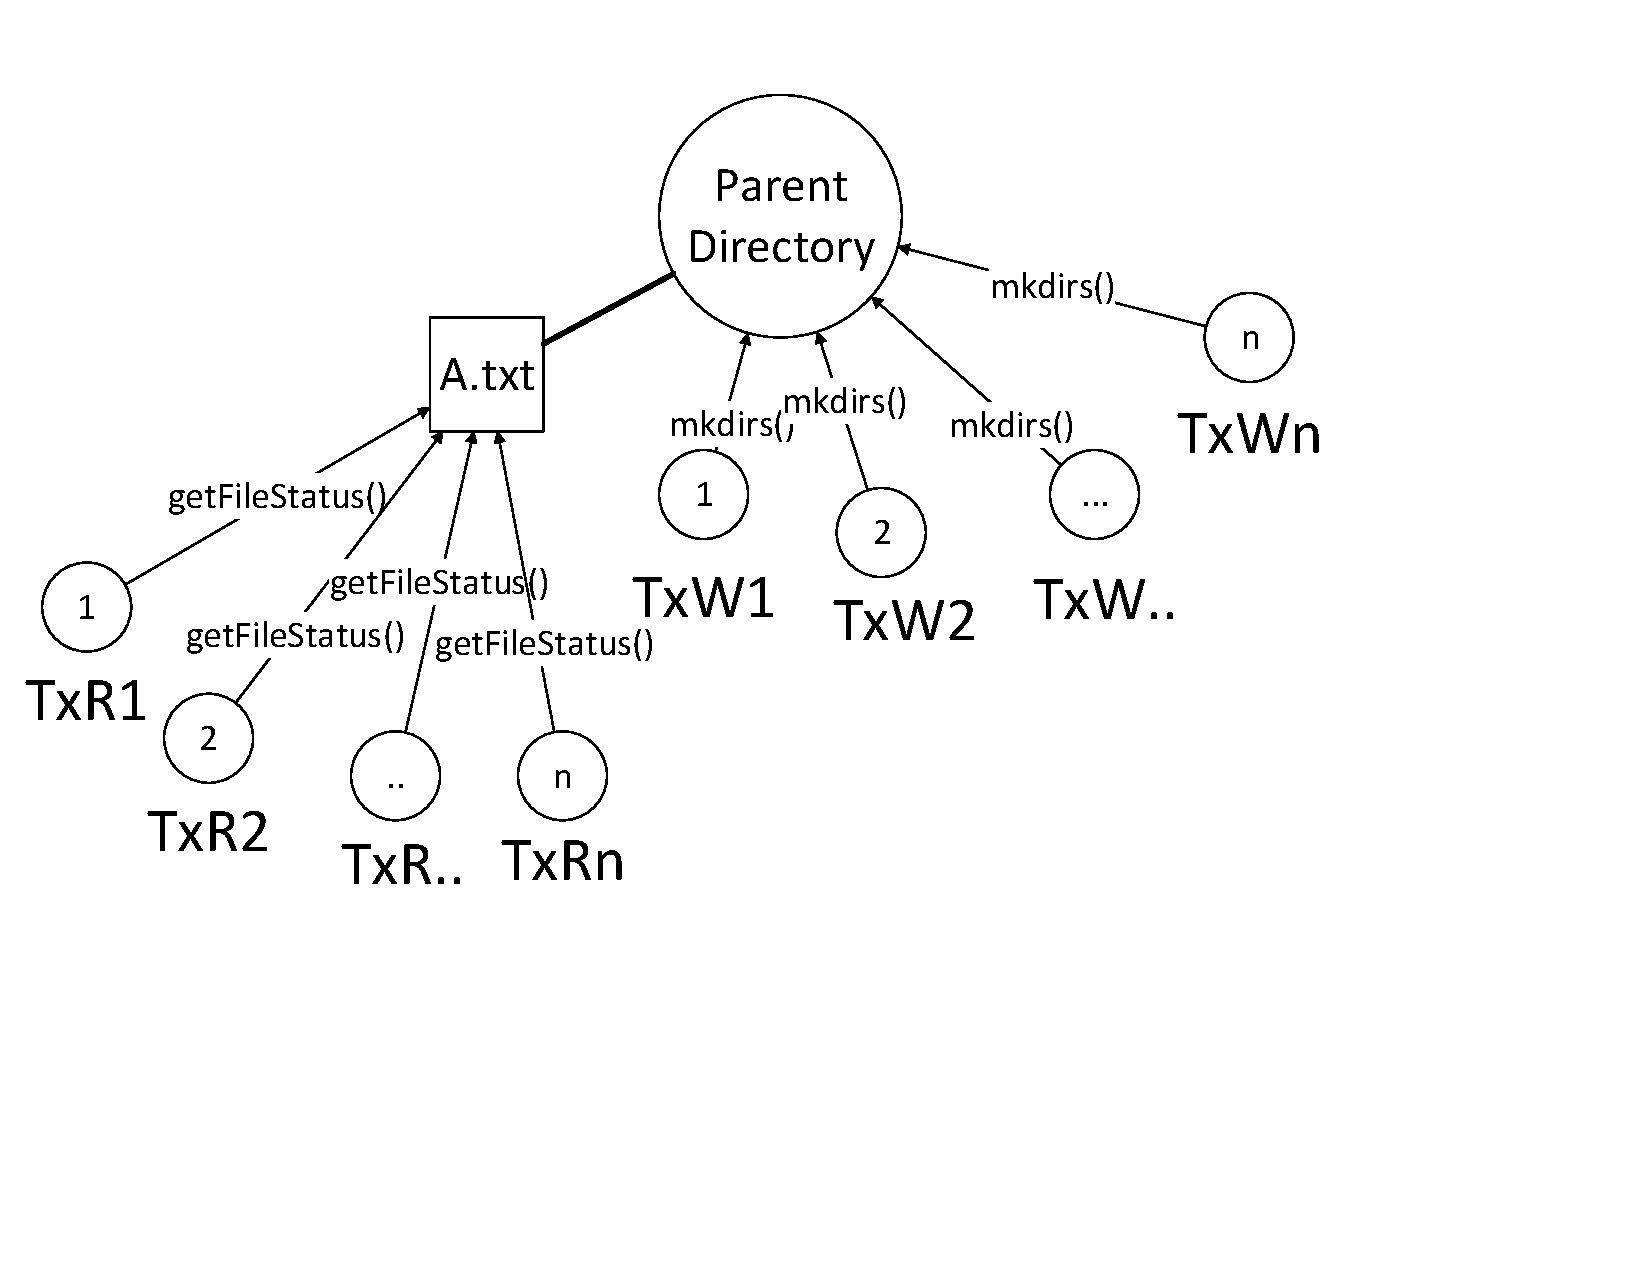
\includegraphics[scale=0.6]{figs/rw.pdf}
	\caption{Read-Write Mixed Workload}
	\label{fig:rwWorkload}
\end{figure}

\noindent From Figure~\ref{fig:rw} and Table~\ref{table:rw}, we can see that OCC still significantly outperforms PCC by 65 \% on this concurrent read-write mixed workload. 

\begin{figure}[ht]
	\centering
	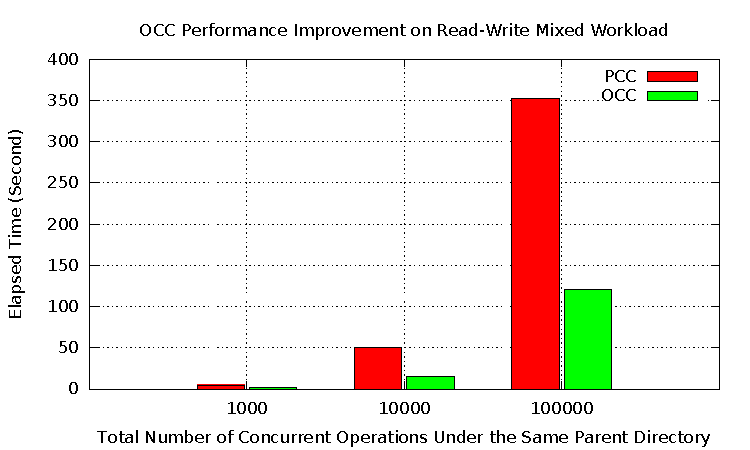
\includegraphics[width=\linewidth]{figs/pcc_occ_rw.pdf}
	\caption{OCC Performance Improvement on Read-Write Mixed Workload}
	\label{fig:rw}
\end{figure}

\begin{table}[ht]
	\centering
	\begin{tabular}{|c|c|c|c|}
		\hline
		\textbf{Num. of Concurrent Creation}                                                 & \textbf{1000}   & \textbf{10000}  & \textbf{100000} \\ \hline
		PCC                                                                                  & 4.92s           & 50.69s          & 352.25s         \\ \hline
		OCC                                                                                  & 1.78s           & 15.31s          & 120.64s         \\ \hline
		\textbf{\begin{tabular}[c]{@{}c@{}}OCC Improvement: \\ (PCC-OCC) / PCC\end{tabular}} & \textbf{63.8\%} & \textbf{69.8\%} & \textbf{65.8\%} \\ \hline
	\end{tabular}
	\caption{OCC Performance Improvement on Read-Write Mixed Workload}
	\label{table:rw}
\end{table}

\section{The Size of Semantic Related Group}

In the read phase and validation phase, we need to fetch the semantic related group. The more levels of directories involved, the more related data rows needs to be fetch. The depth of the path equals to the size of the semantic related group. 
\noindent But since the namespace is a tree structure, the depth of the namespace won't be too much due to the logarithmic order. Also, HDFS limits the maximum number of levels to be 1000, and maximum number of characters for the full path name to be 3000~\footnote{If we assume that 10 characters for one directory name, the maximum level will be 300.}. 

\noindent In addition, batch reading is also used to minimize the network round-trips so that multiple data can fetched in one round-trip. Therefore, the size of semantic related group will not be a limitation in practice. 

\noindent Here we did a test to see how performance affected by different size of semantic related group. Similar to the experiment in Section~\ref{sec:ww}, we have 100 concurrent operations (\textit{mkdirs()}) running under the same parent directory. See Figure~\ref{fig:srg} for the linear relationship between the size and the elapsed time.

\begin{figure}[ht]
	\centering
	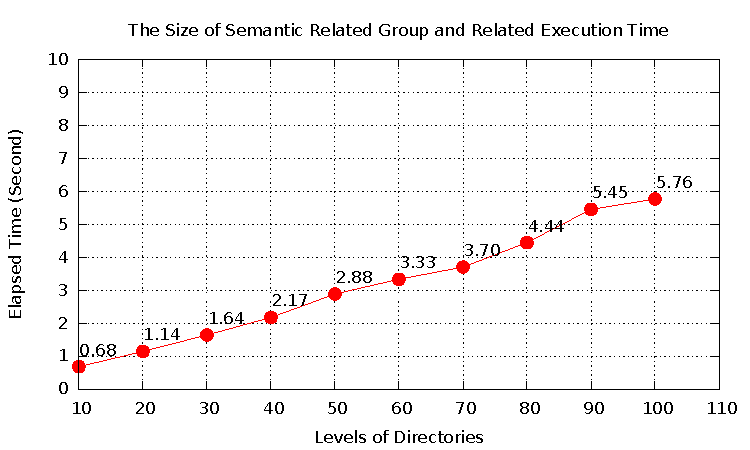
\includegraphics[width=\linewidth]{figs/srgSize.pdf}
	\caption{The Size of Semantic Related Group and Related Execution Time}
	\label{fig:srg}
\end{figure}

\section{OCC Performance with Different Size of Conflicts}

When OCC conflicts happen, transactions will abort, wait for random milliseconds and retry. Eventually one transaction will success, and others will get updated values after retry and return RPC callbacks.

\noindent Here we have 10000 concurrent operations running under the same parent directory. Each operation creates only one sub-directory. Some of them will success and some others will fail due to conflicts. These operations will try to create same sub-directories in different numbers from 1 (100 \% conflicts), to 10000 (0 \% conflicts). Therefore, we have different size of conflicts.

\begin{figure}[ht]
	\centering
	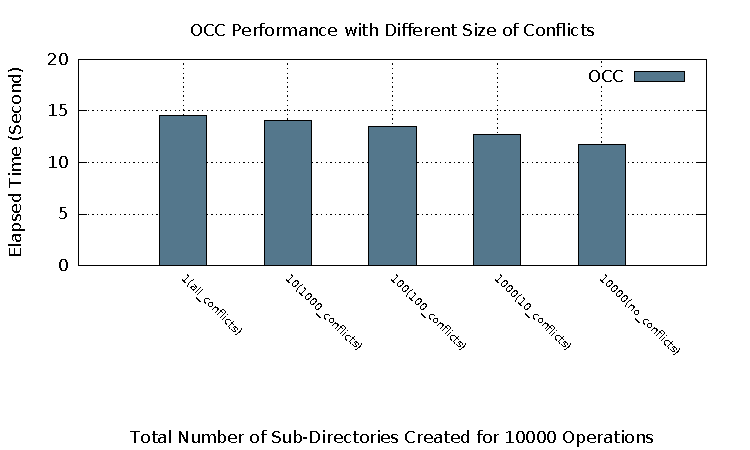
\includegraphics[width=\linewidth]{figs/conflict.pdf}
	\caption{OCC Performance with Different Size of Conflicts}
	\label{fig:conflict}
\end{figure}

\begin{table}[ht]
	\centering
\begin{tabular}{|c|c|c|c|}
	\hline
	\textbf{\begin{tabular}[c]{@{}c@{}}Total Num. of Sub-Directories \\ Created for 10000 Operations\end{tabular}} & \textbf{\begin{tabular}[c]{@{}c@{}}Conflict\\  Size\end{tabular}} & \textbf{\begin{tabular}[c]{@{}c@{}}Elapsed Time\\  (Second)\end{tabular}} & \textbf{\begin{tabular}[c]{@{}c@{}}Performance Decrease\\ Compared to Zero Conflict\end{tabular}} \\ \hline
	1                                                                                                              & 100\%                                                             & 14.53                                                                     & 23.7\%                                                                                            \\ \hline
	10                                                                                                             & 10\%                                                              & 14.11                                                                     & 20.1\%                                                                                            \\ \hline
	100                                                                                                            & 1\%                                                               & 13.51                                                                     & 15.0\%                                                                                            \\ \hline
	1000                                                                                                           & 0.1\%                                                             & 12.72                                                                     & 8.23\%                                                                                            \\ \hline
	10000                                                                                                          & 0\%                                                               & 11.75                                                                     & 0\%                                                                                               \\ \hline
\end{tabular}
	\caption{OCC Performance with Different Size of Conflicts}
	\label{table:conflicts}
\end{table}

\noindent From Figure~\ref{fig:conflict} and Table~\ref{table:conflicts}, we can find that the maximum OCC performance decrease is only 23.7\% when 100 \% of the operations conflict:
\begin{center}
	$(14.53-11.75) \div 11.75 = 23.7\%$
\end{center}

\noindent Besides, with Figure~\ref{fig:conRate}, we find that the OCC performance decrease rate grows very slowly after conflict size 10\%. From conflict size 10\% to conflict size 100 \%, the performance decrease rate only grows from 20.1 \% to 23.7 \%.

\begin{figure}[ht]
	\centering
	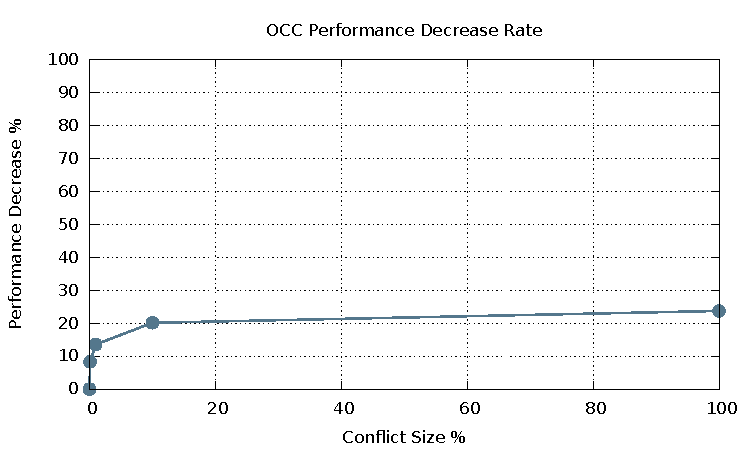
\includegraphics[width=\linewidth]{figs/conRate.pdf}
	\caption{OCC Performance Decrease Rate}
	\label{fig:conRate}
\end{figure}

\section{Correctness Assessment}

The correctness of our OCC implementation for \textit{mkdirs()}~\footnote{other operations are PCC} has been validated by 300+ Apache HDFS 2.0.4 Alpha unit tests passing. The full passing tests list can be found in Appendix~\ref{ch:Testing}.

\section*{Summary}
In this chapter, we gave a detailed evaluation on our OCC solution compared to the previous work on Hop-HDFS (PCC version). We prove that our OCC model performs better than PCC up to \textbf{70 \%} on write-write intense concurrent workload and \textbf{65 \%} on read-write mixed intense concurrent workload. We also evaluated OCC performance decrease on different size of conflict. We find that the maximum OCC performance decrease is only 23.7\% when 100 \% of the operations conflict, and the decrease rate grows very slowly from conflict size 10\% to conflict size 100 \%.